\documentclass[tikz,border=6pt]{standalone}
\usepackage{lmodern}
\usepackage{amsmath}
% Shared macros: residues modulo M drawn on a tilted ring.
\usetikzlibrary{calc,arrows.meta,shadings,fadings}
\definecolor{ablue}{RGB}{38,84,160}
\definecolor{sorange}{RGB}{214,110,22}
\definecolor{ngreen}{RGB}{30,130,76}
\definecolor{ringtop}{RGB}{236,238,242}
\definecolor{ringside}{RGB}{176,182,194}
\newcommand{\RR}{2.15}
\newcommand{\rr}{0.86}
% \ring{M}: the ring centred at the origin of the current scope
\newcommand{\ring}[1]{%
  \shade[left color=ringside!80!black,right color=ringside!80!black,middle color=ringside!55] (-\RR,0) arc[start angle=180,end angle=360,x radius=\RR,y radius=\rr]
     -- (\RR,-0.24) arc[start angle=0,end angle=-180,x radius=\RR,y radius=\rr] -- cycle;
  \draw[ringside!70!black,line width=0.4pt] (-\RR,0) -- (-\RR,-0.24) (\RR,0) -- (\RR,-0.24);
  \draw[ringside!70!black,line width=0.4pt] (\RR,-0.24) arc[start angle=0,end angle=-180,x radius=\RR,y radius=\rr];
  \shade[inner color=white,outer color=ringtop!80!gray] (0,0) ellipse[x radius=\RR,y radius=\rr];
  \draw[ringside!70!black,line width=0.4pt] (0,0) ellipse[x radius=\RR,y radius=\rr];
  \draw[ringside,line width=0.3pt] (0,0) ellipse[x radius=0.80*\RR,y radius=0.80*\rr];
  \foreach \y in {1,...,#1} {%
    \pgfmathsetmacro{\ph}{360*\y/#1}
    \fill[gray!60] ({0.9*\RR*sin(\ph)},{0.9*\rr*cos(\ph)}) circle (0.022);}
  \fill[gray!70] (0,{0.9*\rr}) circle (0.03);
}
% \respos{M}{y}{factor}: coordinate of residue y at radial factor
\newcommand{\respos}[3]{({#3*\RR*sin(360*(#2)/(#1))},{#3*\rr*cos(360*(#2)/(#1))})}
% \elt{M}{y}{colour}: a ball at residue y
\newcommand{\elt}[3]{%
  \pgfmathsetmacro{\sz}{0.085-0.022*cos(360*(#2)/(#1))}
  \shade[ball color=#3] \respos{#1}{#2}{0.9} circle (\sz);}
% \mark{M}{y}{colour}: a hollow marker (a standard multiset) at residue y
\newcommand{\hollow}[3]{%
  \pgfmathsetmacro{\sz}{0.15-0.03*cos(360*(#2)/(#1))}
  \draw[#3,line width=1.1pt] \respos{#1}{#2}{0.9} circle (\sz);}
% \lab{M}{y}{text}: label outside the ring, anchored towards the residue
\newcommand{\lab}[3]{%
  \pgfmathsetmacro{\c}{cos(360*(#2)/(#1))}
  \pgfmathsetmacro{\s}{sin(360*(#2)/(#1))}
  \pgfmathsetmacro{\an}{atan2(-\c,-\s)}
  \pgfmathsetmacro{\dz}{(\c<0)*0.24}
  \node[font=\footnotesize,inner sep=1.5pt,anchor=\an] at ({(\RR+0.08)*\s},{(\rr+0.08)*\c-\dz}) {#3};}

\begin{document}
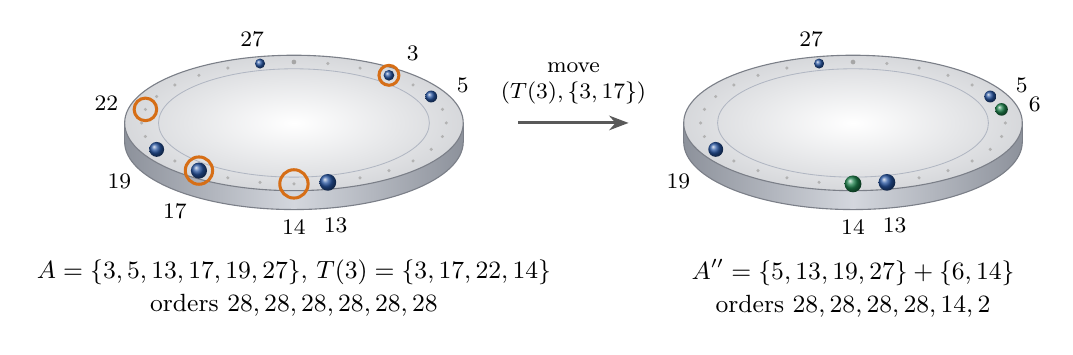
\begin{tikzpicture}
\begin{scope}
  \ring{28}
  \foreach \y in {3,17,22,14} {\hollow{28}{\y}{sorange}}
  \foreach \y in {3,5,13,17,19,27} {\elt{28}{\y}{ablue}}
  \foreach \y in {3,5,13,17,19,27,22,14} {\lab{28}{\y}{$\y$}}
  \node[font=\small,align=center] at (0,-2.1) {$A=\{3,5,13,17,19,27\}$,\ $T(3)=\{3,17,22,14\}$\\[1pt]
     orders $28,28,28,28,28,28$};
\end{scope}
\draw[-{Stealth[length=7pt]},line width=1.1pt,gray!70!black] (2.85,0) -- (4.25,0)
   node[midway,above=3pt,font=\footnotesize,align=center,text=black] {move\\$(T(3),\{3,17\})$};
\begin{scope}[xshift=7.1cm]
  \ring{28}
  \foreach \y in {5,13,19,27} {\elt{28}{\y}{ablue}}
  \foreach \y in {6,14} {\elt{28}{\y}{ngreen}}
  \foreach \y in {5,6,13,14,19,27} {\lab{28}{\y}{$\y$}}
  \node[font=\small,align=center] at (0,-2.1) {$A''=\{5,13,19,27\}+\{6,14\}$\\[1pt]
     orders $28,28,28,28,14,2$};
\end{scope}
\end{tikzpicture}
\end{document}
